

The general model is divided into three main components:
\begin{itemize}
\item Simulation
\item Display
\item Sensor
\end{itemize}

Then there is also two components that are more general classes: \emph{Timestamp} and \emph{Data}. These two classes will be used by the other components, as they are of general purpose.

Figure \ref{meta-meta-model} shows the links between the different components of the general model.

\begin{figure}
  \centering
  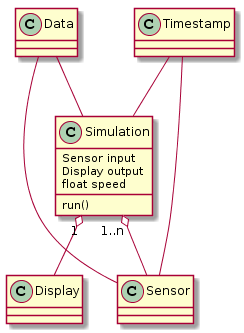
\includegraphics[scale = 0.5]{figures/meta-meta-model.png}
  \label{meta-meta-model}
  \caption{The general model}
\end{figure}

\subsection{Simulation}

The simulation is the core class that will run the simulation. In this class, the user should be able to define the speed at with he wants to run the simulation (for example run a simulation twice as fast as it should be). He will also define the sensors that will be used, and the display where whe wants to output the data. Finally, the method run will launch the simulation.


\subsection{Display}

This class will deal with the output of the simulation. Many different outputs can be defined: CSV, JSON formats, or outputing in an influxDB database (that can be seen with Grafana).


\subsection{Sensor}

This is the most interesting class that will allow the user to define sensors. The sensors here will be defined according to different models, and then they should work all the same way, no matter what is their definition (for example a Markov chain sensor should look the same as a sensor mimicing the data coming from an existing database.


\subsection{Timestamp}

The Timestamp class is here to provide a more friendly interface for time. Time is crucial in the simulation of sensors because the user might want to speed up the simulation, and see if the simulation will be able to print values in real time (to see if the platform is not overloading).


\subsection{Data}

Finally, the Data class will represent the data in memory. This class will not be used by the user but it will be necessary for the application, as it will have to deal with data during computation.








